%**************************************************************************************
% License:
% CC BY-NC-SA 4.0 (http://creativecommons.org/licenses/by-nc-sa/4.0/)
%**************************************************************************************

\documentclass[notes]{beamer}

\mode<presentation> {

\usetheme{Madrid}

% Burnt orange
\definecolor{burntorange}{rgb}{0.8, 0.33, 0.0}
\colorlet{beamer@blendedblue}{burntorange}
% Pale yellow
\definecolor{paleyellow}{rgb}{1.0, 1.0, 0.953}
\setbeamercolor{background canvas}{bg=paleyellow}
% Secondary and tertiary palett
\setbeamercolor*{palette secondary}{use=structure,fg=white,bg=burntorange!80!black}
\setbeamercolor*{palette tertiary}{use=structure,fg=white,bg=burntorange!60!black}

% To remove the footer line in all slides uncomment this line
%\setbeamertemplate{footline}
% To replace the footer line in all slides with a simple slide count uncomment this line
%\setbeamertemplate{footline}[page number]

% To remove the navigation symbols from the bottom of all slides uncomment this line
%\setbeamertemplate{navigation symbols}{}
}

\usepackage{amsmath}
\usepackage{bm}
\usepackage{breqn}
\usepackage{graphicx} % for figures
\usepackage{subcaption} % for subplots 
\usepackage[labelsep=space,tableposition=top]{caption}
\renewcommand{\figurename}{Fig.} 
\usepackage{cleveref}
\usepackage{caption,subcaption}% http://ctan.org/pkg/{caption,subcaption}
\usepackage{booktabs} % Allows the use of \toprule, \midrule and \bottomrule in tables
\usepackage{multirow}

% To print 2 slides on a page
%\usepackage{handoutWithNotes}
%\pgfpagesuselayout{2 on 1}[border shrink=2mm]
%----------------------------------------------------------------------------------------
%	TITLE PAGE
%----------------------------------------------------------------------------------------
% The short title appears at the bottom of every slide, the full title is only on the title page
\title[CE394M: Constitutive Modeling]{CE394M: Constitutive Modeling} 
\author{Krishna Kumar} % name
\institute[UT Austin] % institution 
{
University of Texas at Austin \\
\medskip
\textit{
  \url{krishnak@utexas.edu}} % Your email address
}
\date{\today} % Date, can be changed to a custom date

\begin{document}

\begin{frame}
\titlepage % title page as the first slide
\end{frame}

\begin{frame}
 % Table of contents slide, comment this block out to remove it
 \frametitle{Overview}
  %Throughout your presentation, if you choose to use \section{} and \subsection{} 
  %commands, these %will automatically be printed on this slide as an overview 
 \tableofcontents
\end{frame}

%----------------------------------------------------------------------------------------
% slides
%----------------------------------------------------------------------------------------
\note{
	The objective of constitutive modelling is the determination of stiffness tensor $\mathbf{C}$, a relation between stress and strain tensors.

}
\section{Definition of stress and strain tensors}
%----------------------------------------------------------------------------------------
\begin{frame}
\frametitle{Stresses}
\mode<beamer>{
	\begin{figure}[ht]
	\centering
	\begin{subfigure}[b]{0.49\linewidth}
		\centering
		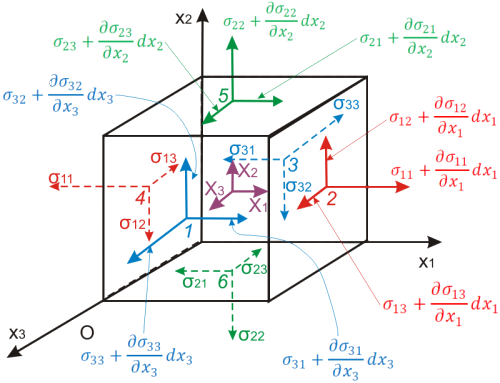
\includegraphics[width=\textwidth]{figs/stress-equilibrium.png}
	\end{subfigure}	
	\begin{subfigure}[b]{0.49\linewidth}
		\centering
		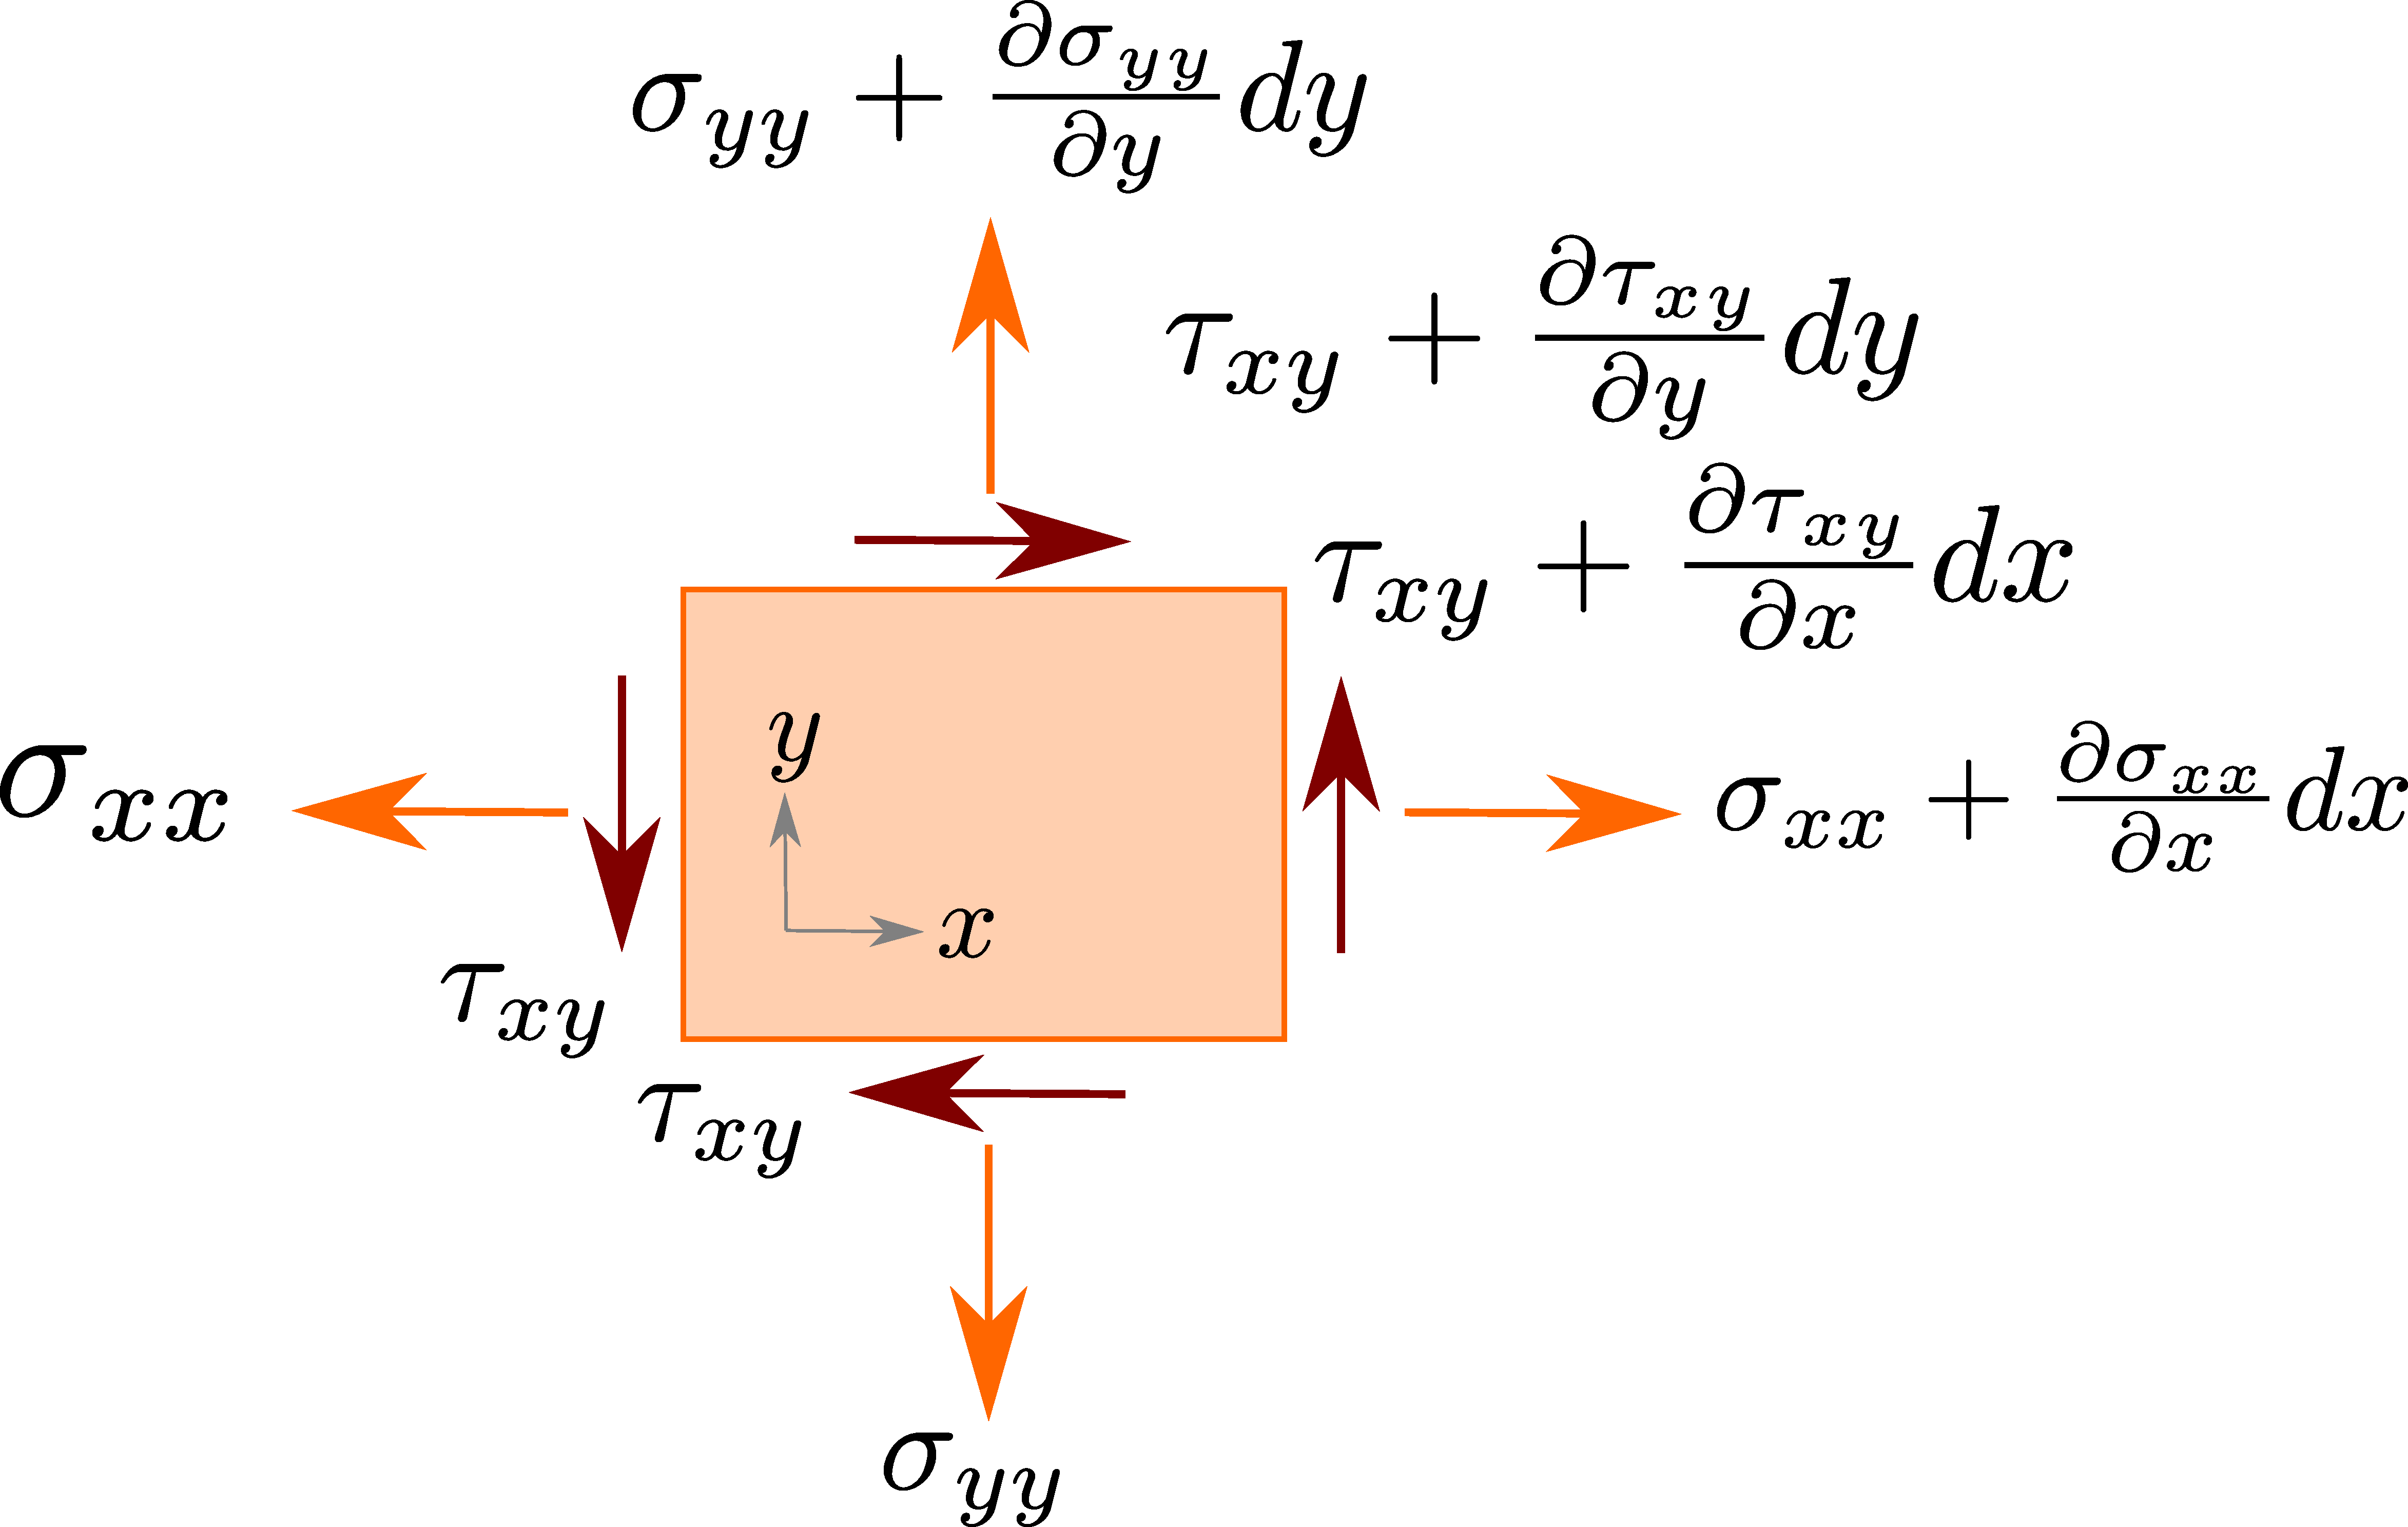
\includegraphics[width=0.85\textwidth]{figs/equilibrium-finished.pdf}
	\end{subfigure}%
\end{figure}
\begin{itemize}
	\item Stress state at a point is defined by $\sigma_{ij}$ in a frame of reference. 
	\item Equilibrium of moments require $sigma_{xz} = \sigma_{zx}, \dots$ etc.,
\end{itemize}
}
\mode<handout>{
	\begin{figure}[ht]
		\centering
		\begin{subfigure}[b]{0.49\linewidth}
			\centering
			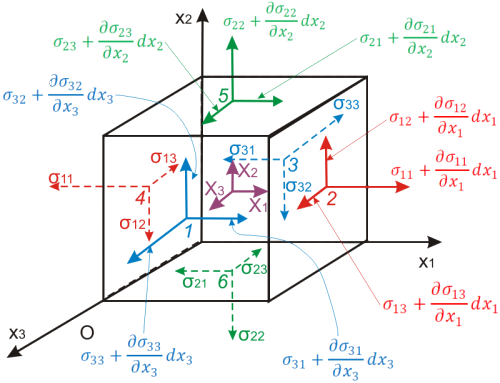
\includegraphics[width=\textwidth]{figs/stress-equilibrium.png}
		\end{subfigure}	
		\begin{subfigure}[b]{0.49\linewidth}
			\centering
			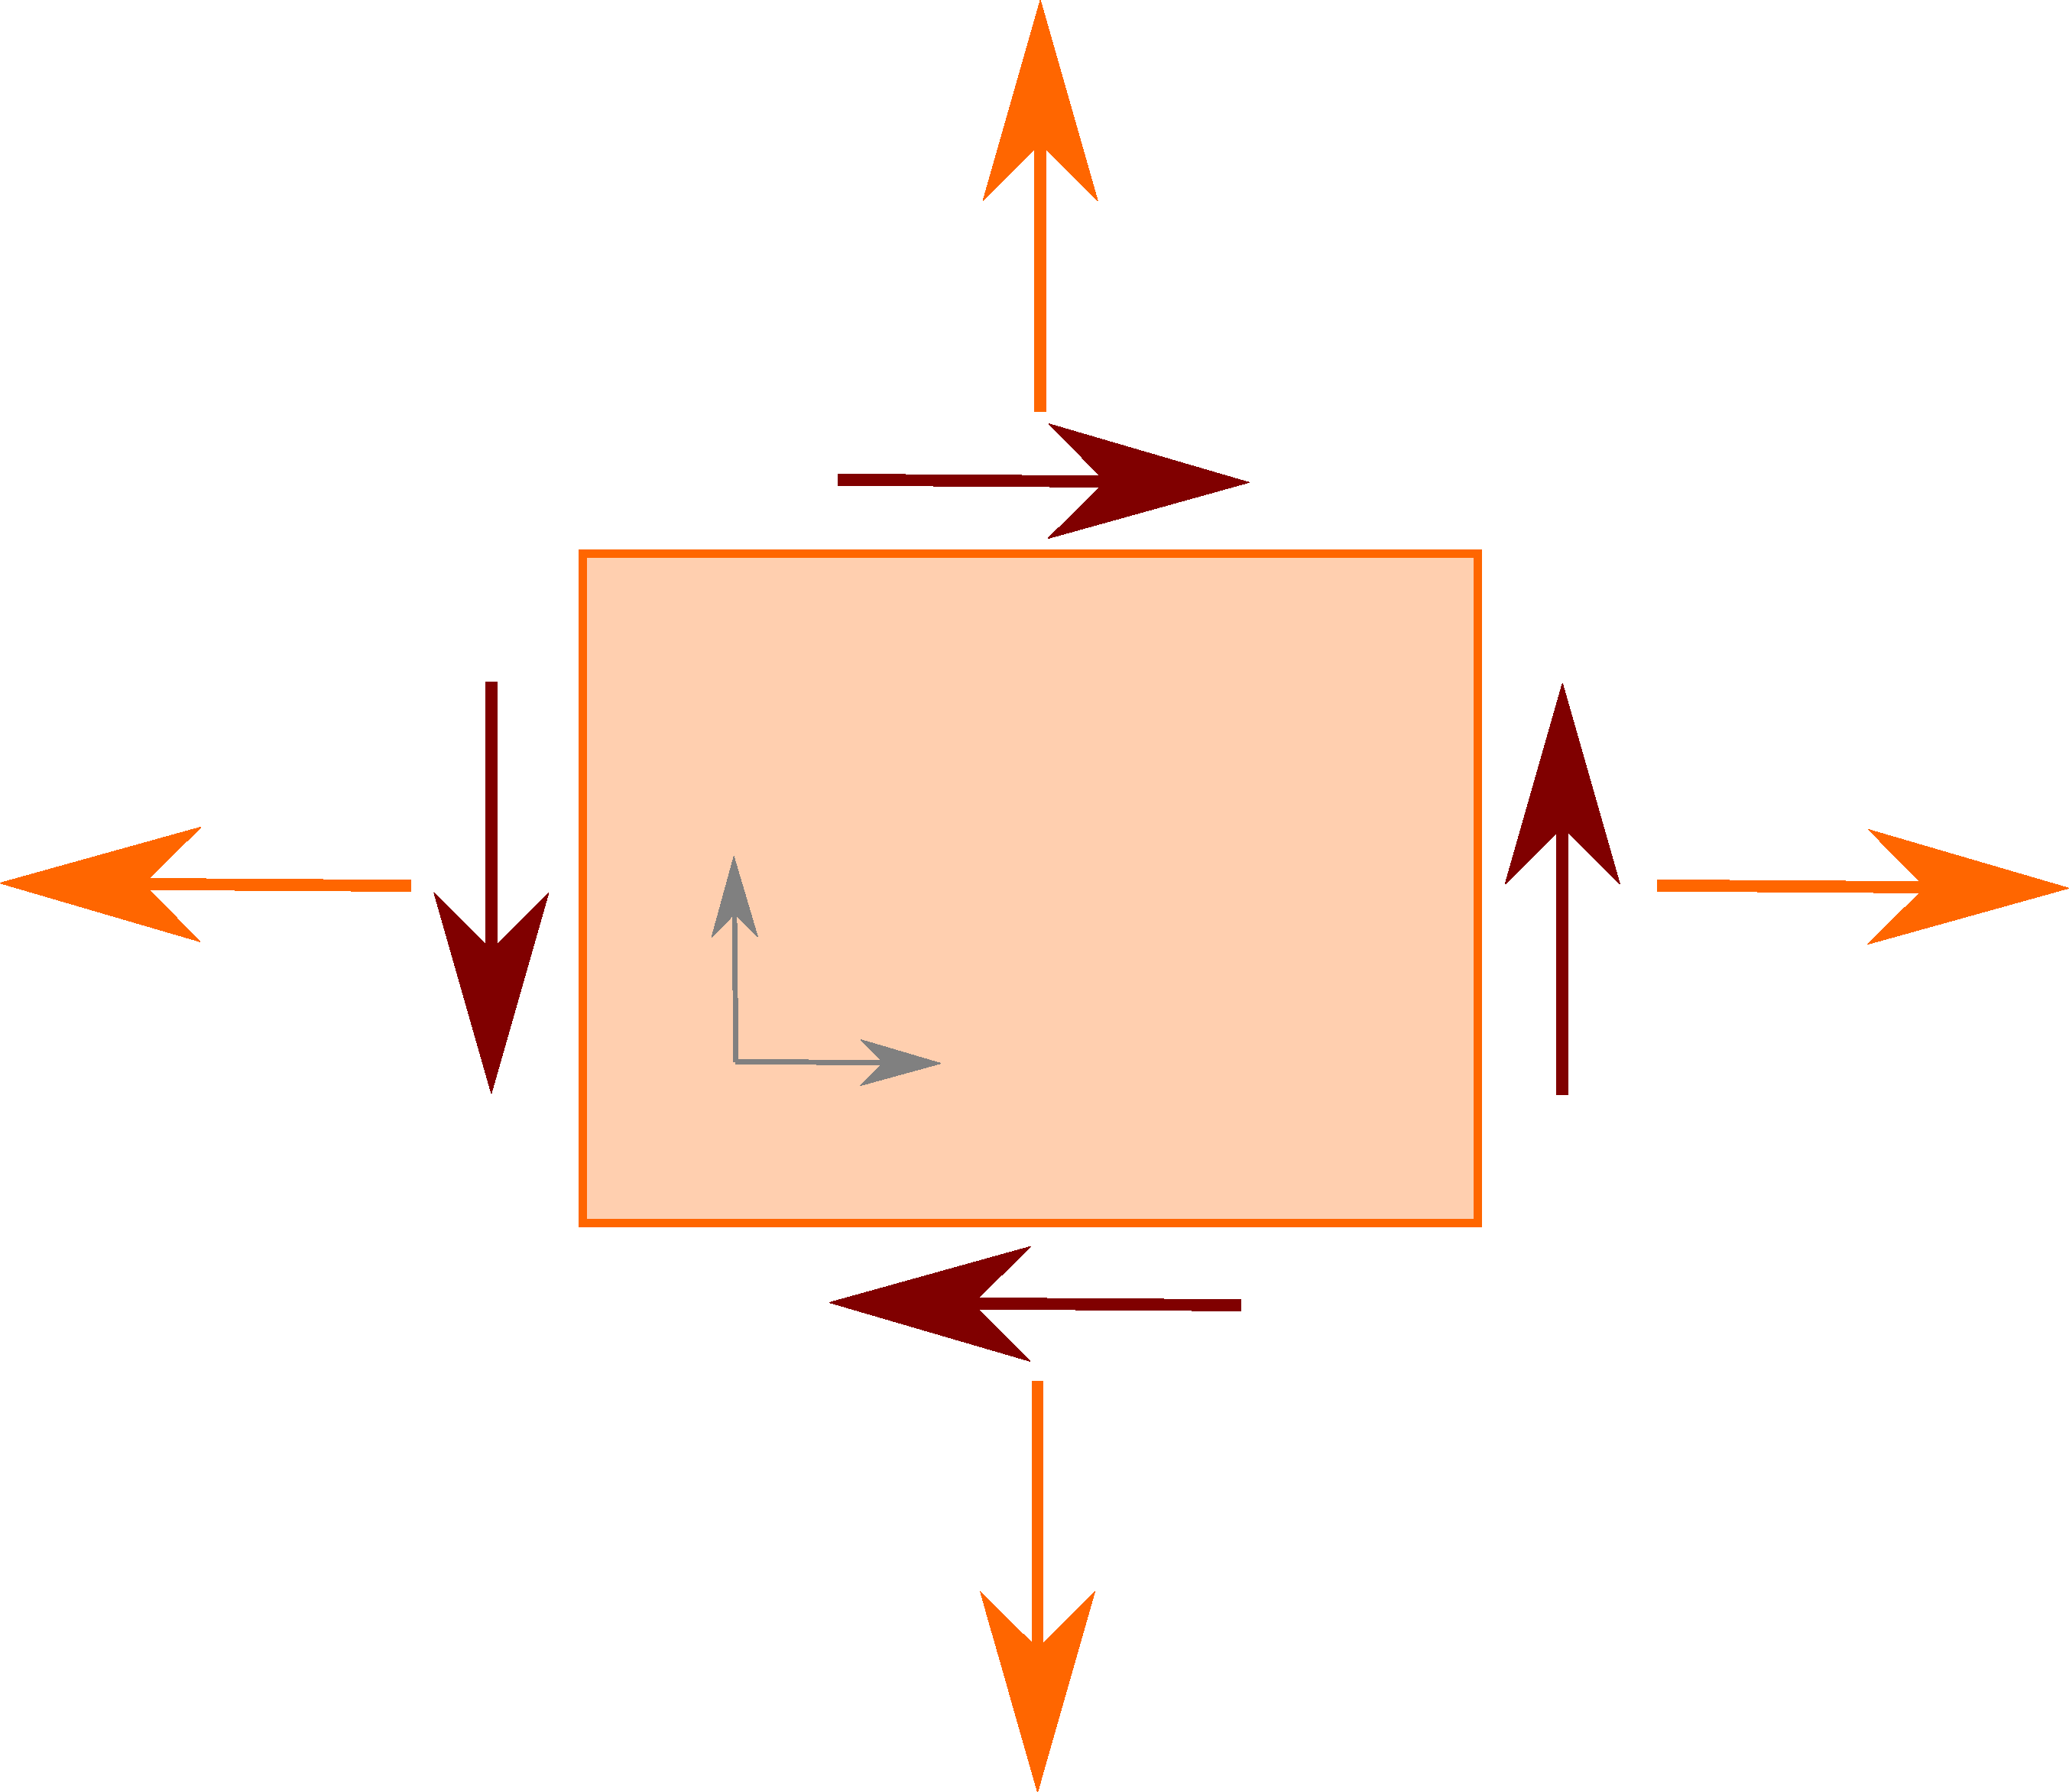
\includegraphics[width=0.85\textwidth]{figs/equilibrium.pdf}
		\end{subfigure}%
	\end{figure}
	\vspace{2cm}
}
\end{frame}
\note{
	\begin{itemize}
		\item $\sigma_{xz}$ stress acting on plane perpendicular to axis $x$ and in the direction of $z$
		\item $\sigma_{xx}$ stress acting on plane perpendicular to axis $x$ and in the direction of $x$
	\end{itemize}

}

%----------------------------------------------------------------------------------------
\begin{frame}
\frametitle{Stresses}
\noindent
\fboxsep=0pt
\noindent
\begin{minipage}[t]{0.59\linewidth}
	\mode<beamer>{	
		\begin{itemize}
			\item 9 components of the stress tensor.
			\item 6 stresses: $\sigma_{11}, \sigma_{22}, \sigma_{33}, \tau_{12}, \tau_{23}, \tau_{31}$.
			\item $\tau_{21} = -\tau_{12}, \tau_{32} = - \tau_{23}, \tau_{13} = - \tau_{31}$
			\item Compression is positive
			\item Shear stress, anti-clockwise is positive
			\item In order to write the components in a more concise way we can use the indices notation: $\sigma_{ij}$ (use $i = 1,2,3$ and $j = 1,2,3$)
			\item Correspondence from $x, y, z$ to $1, 2, 3$ (e.g., $\sigma_{11} = \sigma_{xx}, \sigma_{12} = \sigma_{xy}$)
		\end{itemize}
	}
\end{minipage}%
\hfill%
\begin{minipage}[t]{0.39\linewidth}
	\begin{figure}
		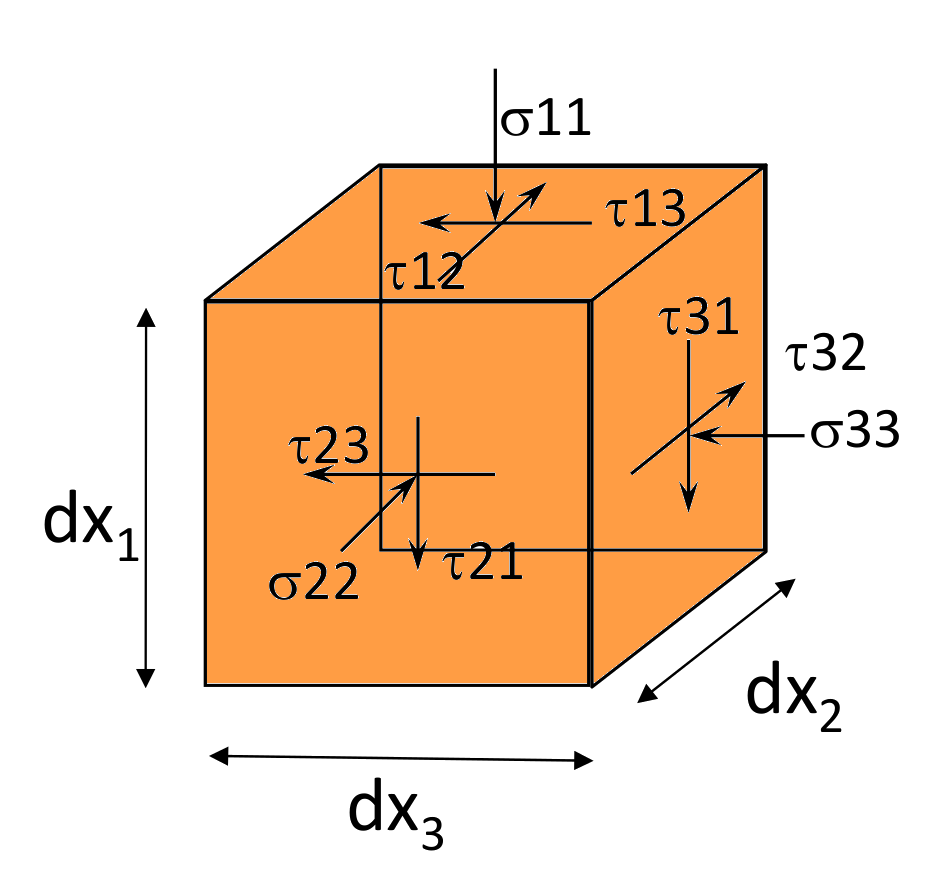
\includegraphics[width=\textwidth]{figs/stresses.png}
	\end{figure}
\end{minipage}	
\end{frame}

%----------------------------------------------------------------------------------------
\begin{frame}
\frametitle{Cauchy stress vs Piola-Kirchoff stress}
\begin{figure}[ht]
	\centering
	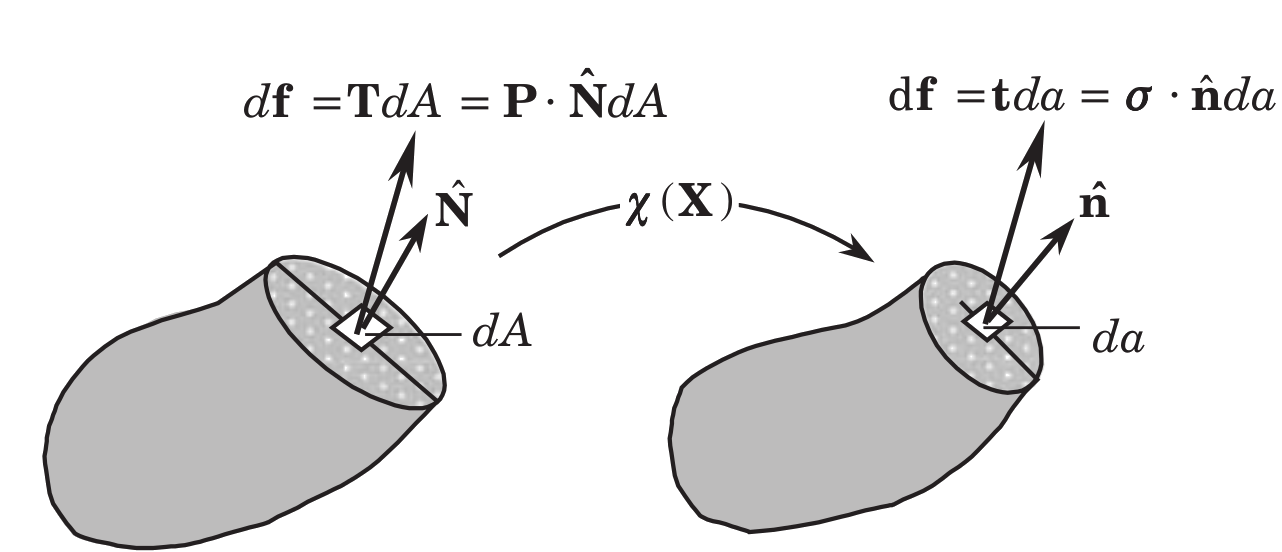
\includegraphics[width=\textwidth]{figs/cauchy-kirchoff-stress-tensor.png}
	\caption*{An introduction to continuum mechanics - J. N. Reddy (2008)}
\end{figure}
\mode<beamer>{
	\begin{itemize}
		\item The first Piola–Kirchhoff stress tensor, also referred to as the \textit{nominal stress tensor},
		or \textit{Lagrangian stress tensor}, gives the current force per unit undeformed area.
	\end{itemize}
}
\mode<handout>{
	\vspace{2cm}
}
\end{frame}
\end{document}